% =====================================================================
%  IoT Mini Project Report: CSA-6401 Internet of Things, Goa University
%  Format: strictly 2 pages, Times, headings 14 pt bold, body 11 pt,
%          line spacing 1.15, margins 0.75 in.
%  Compiles with pdfLaTeX, XeLaTeX or Overleaf (single file).
%  Everything printed in RED is a placeholder: fill it in before submitting.
%  Photos: put figures/prototype.jpg and figures/team.jpg next to this file
%          (optional logo: figures/goa_university_logo.png). They are picked
%          up automatically; until then a framed placeholder is shown.
% =====================================================================
\documentclass[11pt,a4paper]{article}
\usepackage[margin=0.75in]{geometry}
\usepackage{iftex}
\ifPDFTeX
  \usepackage[T1]{fontenc}
  \usepackage{newtxtext,newtxmath}          % Times New Roman clone
\else
  \usepackage{fontspec}
  \setmainfont{texgyretermes}[Extension=.otf, UprightFont=*-regular, BoldFont=*-bold,
                              ItalicFont=*-italic, BoldItalicFont=*-bolditalic]
\fi
\usepackage{setspace}
\usepackage{titlesec}
\usepackage{graphicx}
\usepackage{xcolor}
\usepackage{array}
\usepackage{enumitem}
\usepackage{tikz}
\usetikzlibrary{arrows.meta, fit, backgrounds}

\setstretch{1.15}
\setlength{\parindent}{0pt}
\setlength{\parskip}{1pt}
\pagestyle{empty}
\titleformat{\section}{\fontsize{14}{15}\selectfont\bfseries}{\thesection.}{0.35em}{}
\titlespacing*{\section}{0pt}{2pt}{0.5pt}

\newcommand{\fillin}[1]{\textcolor{red}{[#1]}}
\newcommand{\projtitle}{EDGE-AI FACE RECOGNITION ATTENDANCE SYSTEM ON JETSON NANO WITH A REAL-TIME ADMIN WEB DASHBOARD}
% \photo{file}{height}{placeholder text}
\newcommand{\photo}[3]{%
  \IfFileExists{#1}{\includegraphics[width=\linewidth,height=#2,keepaspectratio]{#1}}%
  {\fcolorbox{gray}{gray!6}{\parbox[c][#2][c]{\dimexpr\linewidth-2\fboxsep-2\fboxrule\relax}{\centering\footnotesize\itshape\textcolor{red}{#3}}}}}

\begin{document}

% =========================== PAGE 1: COVER ===========================
\begin{titlepage}
\centering
\IfFileExists{figures/goa_university_logo.png}{\includegraphics[height=2.8cm]{figures/goa_university_logo.png}\par\vspace{0.5cm}}{}
{\fontsize{22}{26}\selectfont\bfseries GOA UNIVERSITY\par}
\vspace{0.25cm}
{\fontsize{16}{20}\selectfont\bfseries GOA BUSINESS SCHOOL\par}
\vspace{0.1cm}
{\large (Discipline of Computer Science and Technology)\par}
\vspace{1.4cm}
{\fontsize{18}{22}\selectfont\bfseries MINI PROJECT REPORT\par}
\vspace{0.8cm}
{\large \textbf{Subject Code \& Name:} CSA-6401: Internet of Things\par}
\vspace{0.1cm}
{\large \textbf{Academic Year:} 2026--2027\par}
\vspace{1.3cm}
{\large\bfseries PROJECT TITLE:\par}
\vspace{0.3cm}
\fbox{\parbox{0.88\linewidth}{\centering\vspace{8pt}{\fontsize{15}{20}\selectfont\bfseries \projtitle\par}\vspace{8pt}}}\par
\vspace{1.4cm}
{\large\bfseries Submitted By:\par}
\vspace{0.3cm}
{\renewcommand{\arraystretch}{1.6}
\begin{tabular}{|>{\centering\arraybackslash}p{1.6cm}|>{\centering\arraybackslash}p{4.2cm}|p{7.4cm}|}
\hline
\textbf{Sr. No.} & \textbf{Exam Seat Number} & \textbf{Student Name} \\ \hline
1 & \fillin{Seat No.} & \fillin{Student Name} \\ \hline
2 & \fillin{Seat No.} & \fillin{Student Name} \\ \hline
3 & \fillin{Seat No.} & \fillin{Student Name} \\ \hline
4 & \fillin{Seat No.} & \fillin{Student Name} \\ \hline
\end{tabular}\par}
\vfill
{\large\bfseries Under the Guidance of:\par}
\vspace{0.2cm}
{\large \fillin{Faculty Name}\par \fillin{Faculty Designation}\par}
\vspace{0.8cm}
\end{titlepage}

% ============ PAGE 2: PROJECT OVERVIEW & IMPLEMENTATION ============
\section{Project Title}
\textbf{\projtitle}

\section{Problem Statement}
Manual roll-calls waste lecture time and are easy to defeat with proxy attendance, while fingerprint and RFID
systems require physical contact or shareable cards. Cloud face-recognition services transmit student images
over the internet, raising privacy concerns, adding latency and failing when connectivity drops. A contactless,
proxy-resistant system is needed that processes faces locally on an edge device while allowing remote
administration.

\section{Proposed Solution}
A camera at the classroom entrance streams frames to an NVIDIA Jetson Nano. A multi-threaded pipeline detects
faces with a CNN detector on the GPU, tracks them between detections using 68-point facial landmarks, and
identifies them by matching 128-D face encodings against registered members. To prevent printed-photo proxies,
attendance is marked only after a blink is verified via the eye aspect ratio (EAR), logging each member once per
day (name, date, time) to a local CSV file so offline operation remains uninterrupted.

A lightweight Python HTTP server on the Nano exposes a REST API, a Server-Sent Events (SSE) stream and an
MJPEG live preview protected by an API key, published over HTTPS via Cloudflare Tunnel. The online admin
dashboard receives real-time check-ins, unknown-face alerts and device telemetry, and sends commands back to
start/stop tracking, register members via photo upload or Nano camera capture, manage logs and tune settings live.

\section{Hardware \& Software Used}
\begin{itemize}[leftmargin=1.2em, itemsep=0pt, topsep=0pt, parsep=0pt]
  \item \textbf{Microcontroller / Edge Computer:} NVIDIA Jetson Nano Developer Kit \fillin{4 GB} (quad-core ARM
        Cortex-A57, 128-core Maxwell GPU), JetPack \fillin{4.6}, 5 V \fillin{4 A} power supply.
  \item \textbf{Sensors \& Actuators:} \fillin{USB webcam model / Raspberry Pi Camera v2 (CSI)} image
        sensor; HDMI monitor for on-device HUD (outputs are the HUD and web dashboard).
  \item \textbf{Cloud / Platform / Protocols:} HTTP REST, SSE and MJPEG over HTTPS (Cloudflare Tunnel), API-key
        auth, dashboard on \fillin{GitHub Pages / Netlify}; Python 3, OpenCV, dlib, NumPy, HTML/CSS/JS.
\end{itemize}

\section{System Block Diagram}
\vspace{-4pt}
\begin{center}
\resizebox{0.92\linewidth}{!}{%
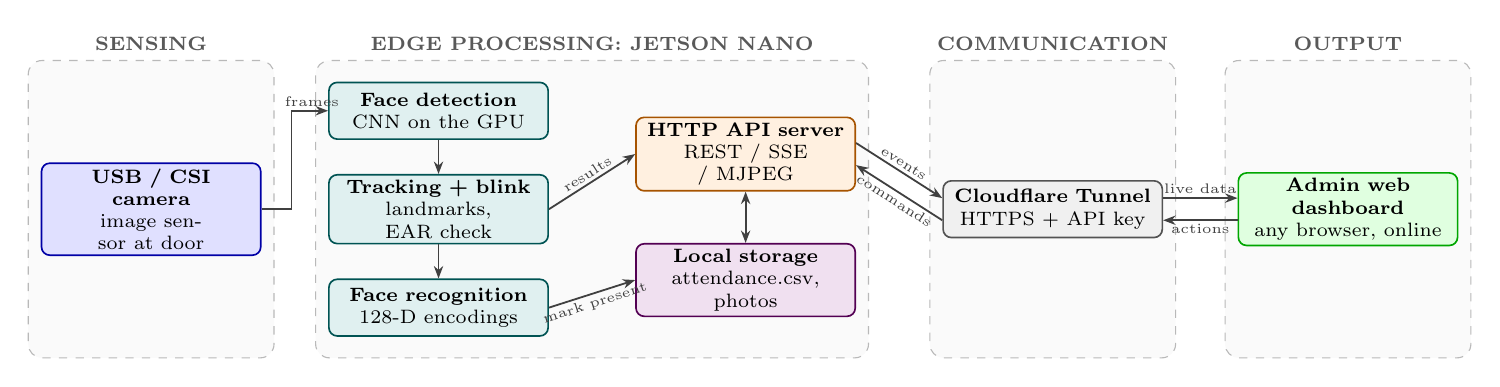
\begin{tikzpicture}[
  font=\scriptsize, >={Stealth[length=4.5pt]},
  blk/.style={draw=#1!65!black, fill=#1!12, rounded corners=3pt, text width=2.55cm, align=center,
              minimum height=0.72cm, inner ysep=2pt, line width=0.6pt},
  lane/.style={draw=gray!55, dashed, fill=gray!4, rounded corners=5pt, inner sep=4.5pt},
  lanelbl/.style={font=\scriptsize\bfseries, text=black!65},
  arr/.style={->, line width=0.65pt, draw=black!75},
  lbl/.style={font=\tiny, text=black!75, inner sep=1.2pt}]
  % blocks
  \node[blk=blue]   (cam)  at (0,-1.25)    {\textbf{USB / CSI camera}\\image sensor at door};
  \node[blk=teal]   (det)  at (3.65,0)     {\textbf{Face detection}\\CNN on the GPU};
  \node[blk=teal]   (trk)  at (3.65,-1.25) {\textbf{Tracking + blink}\\landmarks, EAR check};
  \node[blk=teal]   (rec)  at (3.65,-2.50) {\textbf{Face recognition}\\128-D encodings};
  \node[blk=orange] (srv)  at (7.55,-0.55) {\textbf{HTTP API server}\\REST / SSE / MJPEG};
  \node[blk=violet] (csv)  at (7.55,-2.15) {\textbf{Local storage}\\attendance.csv, photos};
  \node[blk=gray]   (tun)  at (11.45,-1.25){\textbf{Cloudflare Tunnel}\\HTTPS + API key};
  \node[blk=green]  (dash) at (15.2,-1.25) {\textbf{Admin web dashboard}\\any browser, online};
  % lanes (Sensors -> Edge device -> Communication -> Output)
  \coordinate (T) at (0,0.48); \coordinate (B) at (0,-2.98);
  \begin{scope}[on background layer]
    \node[lane, fit=(cam)(cam|-T)(cam|-B), label={[lanelbl]above:SENSING}] {};
    \node[lane, fit=(det)(rec)(srv)(csv)(det|-T)(det|-B), label={[lanelbl]above:EDGE PROCESSING: JETSON NANO}] {};
    \node[lane, fit=(tun)(tun|-T)(tun|-B), label={[lanelbl]above:COMMUNICATION}] {};
    \node[lane, fit=(dash)(dash|-T)(dash|-B), label={[lanelbl]above:OUTPUT}] {};
  \end{scope}
  % data flow
  \draw[arr] (cam.east) -- ++(0.38,0) |- node[lbl, pos=0.78, above]{frames} (det.west);
  \draw[arr] (det) -- (trk);
  \draw[arr] (trk) -- (rec);
  \draw[arr] (rec.east) -- node[lbl, below, sloped]{mark present} (csv.west);
  \draw[arr] (trk.east) -- node[lbl, above, sloped]{results} (srv.west);
  \draw[arr, <->] (srv) -- (csv);
  \draw[arr] ([yshift=4pt]srv.east) -- node[lbl, above, sloped]{events} ([yshift=4pt]tun.west);
  \draw[arr] ([yshift=-4pt]tun.west) -- node[lbl, below, sloped]{commands} ([yshift=-4pt]srv.east);
  \draw[arr] ([yshift=4pt]tun.east) -- node[lbl, above]{live data} ([yshift=4pt]dash.west);
  \draw[arr] ([yshift=-4pt]dash.west) -- node[lbl, below]{actions} ([yshift=-4pt]tun.east);
\end{tikzpicture}}
\end{center}
\vspace{-8pt}

\section{Project \& Team Photographs}
\begin{minipage}[t]{0.485\linewidth}\centering
  \textbf{\small Photo 1: Working Hardware Prototype}\par\vspace{1.5pt}
  \photo{figures/prototype.jpg}{2.05cm}{Insert close-up of Jetson Nano, camera \& dashboard screen (figures/prototype.jpg)}
\end{minipage}\hfill
\begin{minipage}[t]{0.485\linewidth}\centering
  \textbf{\small Photo 2: Group Members with Project}\par\vspace{1.5pt}
  \photo{figures/team.jpg}{2.05cm}{Insert group photo of team members standing with the working model (figures/team.jpg)}
\end{minipage}

\section{Conclusion / Future Scope}
The prototype met its objective: it recognises registered members at the door, blocks printed-photo proxies
with blink detection and streams attendance to the online dashboard in real time at \fillin{X} FPS on the
Jetson Nano. A practical upgrade is a TensorRT detector with MQTT/cloud-DB sync across multiple classrooms.

\end{document}
